\documentclass[aspectratio=169,10pt]{beamer}

\usetheme{Madrid}
\usecolortheme{default}
\usefonttheme{professionalfonts}

\usepackage{fontspec}
\setmainfont{Segoe UI}
\setsansfont{Segoe UI}
\usepackage{booktabs}
\usepackage{graphicx}
\usepackage{amsmath}
\usepackage{xcolor}
\usepackage{array}

\definecolor{NavyPrimary}{RGB}{20, 48, 92}
\definecolor{TealAccent}{RGB}{13, 128, 128}
\definecolor{SoftBg}{RGB}{244, 247, 252}
\definecolor{WarmOrange}{RGB}{196, 88, 22}

\setbeamercolor{palette primary}{bg=NavyPrimary,fg=white}
\setbeamercolor{palette secondary}{bg=TealAccent,fg=white}
\setbeamercolor{palette tertiary}{bg=NavyPrimary,fg=white}
\setbeamercolor{structure}{fg=NavyPrimary}
\setbeamercolor{frametitle}{bg=NavyPrimary,fg=white}
\setbeamercolor{block title}{bg=NavyPrimary,fg=white}
\setbeamercolor{block body}{bg=SoftBg,fg=black}
\setbeamercolor{block title example}{bg=TealAccent,fg=white}
\setbeamercolor{block body example}{bg=SoftBg,fg=black}
\setbeamercolor{block title alerted}{bg=WarmOrange,fg=white}
\setbeamercolor{block body alerted}{bg=SoftBg,fg=black}

\setbeamertemplate{navigation symbols}{}
\setbeamertemplate{footline}[frame number]

\title[Hybrid-v4 (V4-4): Neural Codec-Bypass]{\textbf{Hybrid-v4 (\texttt{V4-4}): Kiến Trúc Neural Codec-Bypass Siêu Nhẹ}\\ \large Giải Thích Kiến Trúc \& Từng Module Bên Trong (\texttt{1,95M} Tham Số)}
\author{Nhóm Tái Lập \& Mở Rộng SonicMaster}
\date{Ngày 23 tháng 11 năm 2026}

\begin{document}

%---------------------------------------------------------
\begin{frame}
  \titlepage
\end{frame}

%---------------------------------------------------------
\begin{frame}{1. Động Lực: Từ Hybrid-v3 Tới Hybrid-v4}
  \begin{columns}[T]
    \begin{column}{0.49\textwidth}
      \footnotesize
      \begin{block}{Hạn chế của SonicMaster ($A_0$) \& Hybrid-v3}
        \begin{itemize}
          \item \textbf{SonicMaster ($A_0$):} Hiểu prompt, sửa được cả \texttt{reverb}, \texttt{clip}, \texttt{xband}, nhưng đi qua \textbf{VAE ($21{,}53\text{ Hz}$)} làm mờ chi tiết (\texttt{SSIM} $\approx 0{,}61$) và giọng hát hơi ``kim loại''.
          \item \textbf{Hybrid-v3:} Dùng DSP truyền thống nên rất sạch cho nhóm tuyến tính, nhưng \textbf{cần nhãn lỗi} để phân nhánh và phải \textbf{fallback về $A_0$} ở 64\% ca phi tuyến.
        \end{itemize}
      \end{block}
    \end{column}
    \begin{column}{0.48\textwidth}
      \footnotesize
      \begin{exampleblock}{Ý tưởng vàng của Hybrid-v4 (\texttt{1,95M} tham số)}
        \begin{itemize}
          \item \textbf{Không cần nhãn lỗi}, chạy 100\% tự động từ cặp $(x, s)$.
          \item Xem đầu ra SonicMaster $s$ như \textbf{``kim chỉ nam'' (teacher guide)}.
          \item Mạng neural nhẹ học cách \textbf{lọc trực tiếp trên sóng gốc $x$} (không qua VAE), và tự mở cổng lấy phần thiếu từ $s$ hoặc tổng hợp phần dư phức tại các vùng $x$ bị hỏng nặng.
        \end{itemize}
      \end{exampleblock}
    \end{column}
  \end{columns}
  \vspace{0.4em}
  \centering
  \footnotesize
  \begin{tabular}{lcccc}
    \toprule
    \textbf{Thông số \texttt{V4-4}} & \textbf{Encoder} & \textbf{Backbone (4 Blocks)} & \textbf{Decoder} & \textbf{Tổng tham số} \\
    \midrule
    Số lượng tham số & 553.824 & 433.152 & 966.094 & \textbf{1.953.070 (\textasciitilde 1,95M)} \\
    \bottomrule
  \end{tabular}
\end{frame}

%---------------------------------------------------------
\begin{frame}{2. Sơ Đồ Kiến Trúc Tổng Thể Hybrid-v4}
  \begin{columns}[c]
    \begin{column}{0.60\textwidth}
      \centering
      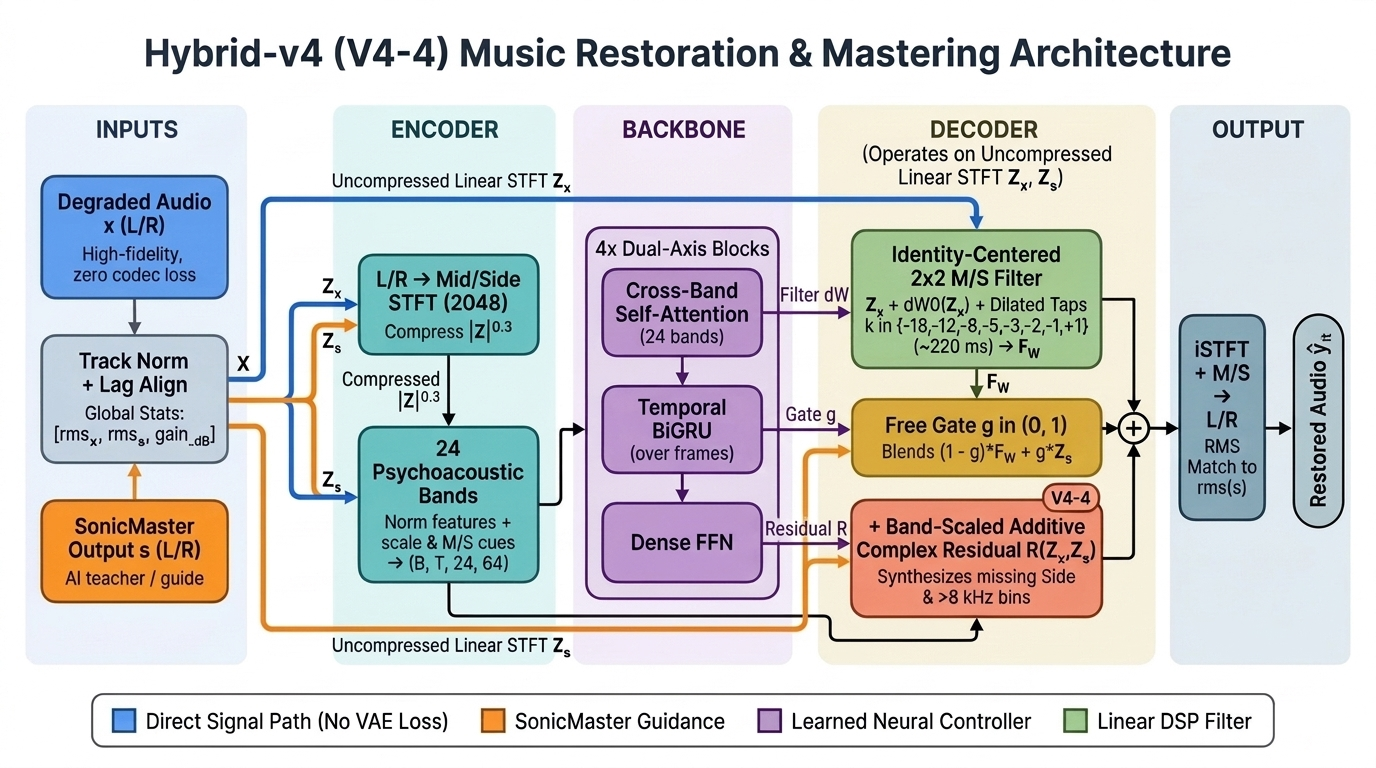
\includegraphics[width=\textwidth,height=0.75\textheight,keepaspectratio]{artifacts/10_extension/figures/hybrid_v4_architecture.jpg}
    \end{column}
    \begin{column}{0.38\textwidth}
      \scriptsize
      \begin{block}{Luồng xử lý 5 module}
        \begin{enumerate}
          \item \textbf{Track Norm + M/S STFT:} Căn độ trễ, chuẩn hóa RMS toàn bài, tách kênh \texttt{Mid/Side} và biến đổi STFT ($1.025$ bin).
          \item \textbf{Psychoacoustic Band Encoder:} Gom thành 24 dải theo tai người $\rightarrow$ tensor $(B, T, 24, 64)$.
          \item \textbf{4 $\times$ DualAxisBlock:} Attention theo dải tần + BiGRU theo thời gian + FFN.
          \item \textbf{Decoder (\texttt{V4-4}):} Lọc phức đa khung giãn cách (\texttt{MF9}) + Cổng tự do (\texttt{Free Gate}) + Phần dư phức (\texttt{Additive Residual}).
          \item \textbf{iSTFT + OLA + RMS Match:} Tái tạo sóng 44,1 kHz stereo khớp âm lượng $s$.
        \end{enumerate}
      \end{block}
    \end{column}
  \end{columns}
\end{frame}

%---------------------------------------------------------
\begin{frame}{3. Module 1: Tiền Xử Lý — Track Norm, Lag Align \& Mid/Side STFT}
  \footnotesize
  \begin{columns}[T]
    \begin{column}{0.48\textwidth}
      \begin{block}{1. Căn trễ \& Chuẩn hóa toàn bài (\texttt{compute\_track\_norm})}
        \begin{itemize}
          \item \textbf{Lag Align:} Căn độ trễ mẫu giữa $s$ và $x$ để 2 sóng khớp nhau từng mẫu âm thanh.
          \item \textbf{Track Norm:} Đưa $x$ và $s$ về cùng thang đo $\text{RMS}(s)$ với hệ số căn $g_{\text{align}}$ giới hạn trong $[-24, +24]\text{ dB}$.
          \item \textbf{3 thống kê toàn bài (\texttt{raw\_stats}):} Lưu lại $(\log \text{RMS}_x,\; \log \text{RMS}_s,\; \Delta\text{dB})$ để mạng không bị ``mù âm lượng''.
        \end{itemize}
      \end{block}
    \end{column}
    \begin{column}{0.49\textwidth}
      \begin{exampleblock}{2. Tách Mid/Side \& Biến đổi STFT}
        \begin{itemize}
          \item \textbf{\texttt{lr\_to\_ms}:} $\text{Mid} = \frac{L+R}{\sqrt{2}}$ (giọng hát, bass, trống giữa), $\text{Side} = \frac{L-R}{\sqrt{2}}$ (không gian 2 tai). Giúp kiểm soát trực tiếp độ rộng stereo.
          \item \textbf{STFT tuyến tính:} \texttt{n\_fft=2048, hop=512} $\rightarrow$ $F=1.025$ bin tần số (~11,6 ms/khung) giữ nguyên để Decoder lọc trực tiếp.
          \item \textbf{Nén biên độ $|Z|^{0{,}3}$ cho Encoder:} Giúp Encoder nhìn rõ dải cao có năng lượng nhỏ hơn bass.
        \end{itemize}
      \end{exampleblock}
    \end{column}
  \end{columns}
\end{frame}

%---------------------------------------------------------
\begin{frame}{4. Module 2: \texttt{PsychoacousticBandEncoder} (24 Dải Tâm Âm Học)}
  \footnotesize
  \begin{block}{Vì sao chia 24 dải không đều (\texttt{BAND\_WIDTHS})?}
    Tai người nghe rất tinh ở dải trầm/trung ($0\text{--}4\text{ kHz}$) và thô dần ở dải cao ($4\text{--}22\text{ kHz}$). Chia $1.025$ bin STFT thành \textbf{24 dải không chồng lấn} (kiểu BSRNN) giúp giảm mạnh chi phí tính toán mà vẫn giữ độ phân giải cao ở vùng giọng hát:
    \begin{itemize}
      \item $0 \text{--} 1.012\text{ Hz}$: 8 dải (chỉ $5\text{--}6\text{ bin}$/dải) \quad $\bullet$ \quad $1.012 \text{--} 4.005\text{ Hz}$: 8 dải ($17\text{--}18\text{ bin}$/dải)
      \item $4.005 \text{--} 12.015\text{ Hz}$: 5 dải ($74\text{--}75\text{ bin}$/dải) \quad $\bullet$ \quad $12.015 \text{--} 22.050\text{ Hz}$: 3 dải ($155\text{--}156\text{ bin}$/dải)
    \end{itemize}
  \end{block}
  \begin{exampleblock}{Dual Scale-Aware Conditioning (Chuẩn hóa kép theo từng dải)}
    Tại mỗi dải $b$ và khung $t$, tách riêng \textbf{hình dạng phổ} (chia cho $\text{RMS}_{b,t}$) và \textbf{thang đo năng lượng}:
    \begin{itemize}
      \item \textbf{Đặc trưng hình dạng ($8 \cdot w_b$ chiều):} Phần thực/ảo chuẩn hóa của $Z_{x,b}$ và $Z_{s,b}$ trên cả 2 kênh $(M, S)$.
      \item \textbf{7 đặc trưng thang đo:} $\log r_{x,b}$, $\log r_{s,b}$, $\log(r_{s,b}/r_{x,b})$, chênh độ rộng stereo $(ms_s - ms_x)$, và 3 số \texttt{raw\_stats}.
      \item Chiếu qua \texttt{LayerNorm + Linear + SiLU} $\rightarrow$ đầu ra \textbf{$(B, T, 24, 64)$}.
    \end{itemize}
  \end{exampleblock}
\end{frame}

%---------------------------------------------------------
\begin{frame}{5. Module 3: Backbone \texttt{4 $\times$ DualAxisBlock} (433K Tham Số)}
  \footnotesize
  Mỗi block (trong 4 block nối tiếp) xử lý tensor $(B, T, 24, 64)$ theo \textbf{2 trục vuông góc} để nắm bắt cả tương quan phổ tức thời lẫn biến thiên theo thời gian:
  \vspace{0.3em}
  \begin{columns}[T]
    \begin{column}{0.32\textwidth}
      \begin{block}{1. Trục Tần số}
        \textbf{\texttt{Cross-Band Self-Attention}} (4 heads, 24 dải):
        \begin{itemize}
          \item Tại cùng 1 thời điểm $t$, 24 dải tần trao đổi thông tin với nhau.
          \item Giúp học quy luật cân bằng màu âm toàn phổ (EQ, \texttt{warm}, \texttt{bright}, \texttt{mud}).
        \end{itemize}
      \end{block}
    \end{column}
    \begin{column}{0.32\textwidth}
      \begin{exampleblock}{2. Trục Thời gian}
        \textbf{\texttt{Temporal BiGRU}} (hai chiều):
        \begin{itemize}
          \item Tại từng dải tần $b$, quét xuyên suốt quá khứ và tương lai.
          \item Phân biệt được tiếng gõ ngắn (transient) với đuôi vang phòng (\texttt{reverb}) kéo dài.
        \end{itemize}
      \end{exampleblock}
    \end{column}
    \begin{column}{0.32\textwidth}
      \begin{block}{3. Tổng hợp phi tuyến}
        \textbf{\texttt{Dense FFN}} ($64 \rightarrow 256 \rightarrow 64$, GELU):
        \begin{itemize}
          \item Đều có \texttt{LayerNorm} trước mỗi nhánh + kết nối tắt (residual).
          \item Tổng hợp đặc trưng đưa sang Decoder.
        \end{itemize}
      \end{block}
    \end{column}
  \end{columns}
\end{frame}

%---------------------------------------------------------
\begin{frame}{6. Module 4: Decoder Của \texttt{V4-4} — Trái Tim Của Kiến Trúc}
  \footnotesize
  \begin{block}{Công thức tổng hợp trên STFT phức tuyến tính (\texttt{MF7Decoder} bản \texttt{V4-4})}
    $$\hat{Z} = (1 - g) \odot \underbrace{\Bigl(Z_x + \Delta W_0(Z_x) + \sum_{k \in \text{MF9}} \Delta W_k(Z_{x,\, t+k})\Bigr)}_{F_W:\text{ Lọc phức 2}\times\text{2 quanh } Z_x} \;+\; g \odot Z_s \;+\; \underbrace{R_\theta(Z_x, Z_s)}_{\text{Điểm mới của V4-4}}$$
  \end{block}
  \begin{columns}[T]
    \begin{column}{0.48\textwidth}
      \begin{exampleblock}{3 thành phần kế thừa từ \texttt{V4-2} / \texttt{V4-3}}
        \begin{itemize}
          \item \textbf{Identity-Centered $2\times 2$ M/S:} Mỗi $\Delta W$ là ma trận phức $2\times 2$ trên $(M, S)$ $\rightarrow$ vừa chỉnh biên độ/pha, vừa trộn chéo $M \leftrightarrow S$ (zero-init quanh $Z_x$).
          \item \textbf{Dilated MF9 (~220 ms):} 9 tap giãn cách $\{-18,-12,-8,-5,-3,-2,-1,0,+1\}$ (chia 96 sub-band) bắt được đuôi reverb dài kiểu WPE.
          \item \textbf{Free Gate ($g \in (0,1)$):} \texttt{gate\_bias=-1.5}, không phạt $\lambda_g$, tự mở để mượn $Z_s$ khi $x$ hỏng nặng.
        \end{itemize}
      \end{exampleblock}
    \end{column}
    \begin{column}{0.49\textwidth}
      \begin{alertblock}{Điểm nâng cấp cốt lõi của \texttt{V4-4}: $R_\theta(Z_x, Z_s)$}
        \begin{itemize}
          \item \textbf{Vấn đề của \texttt{V4-3}:} Khi $x$ bị sụp kênh Side ($S_x \approx 0$, lỗi \texttt{stereo}) hoặc mất sạch dải cao (lỗi \texttt{bright}), phép nhân $\Delta W \cdot Z_x$ bằng $0$, còn $g \cdot Z_s$ chỉ nhân thực nên không sửa được pha của $Z_s$.
          \item \textbf{Giải pháp \texttt{V4-4}:} Mỗi bin xuất thêm 4 kênh cộng trực tiếp $R_\theta = \text{complex}(\cdot) \times \text{band\_rms}$ (scale theo RMS từng dải, zero-init) $\rightarrow$ tổng hợp trực tiếp thành phần phức còn thiếu cho kênh Side \& dải cao.
        \end{itemize}
      \end{alertblock}
    \end{column}
  \end{columns}
\end{frame}

%---------------------------------------------------------
\begin{frame}{7. Module 5: Tái Tạo Sóng Âm, Hàm Loss \& Tiến Hóa \texttt{V4-0} $\rightarrow$ \texttt{V4-4}}
  \begin{columns}[T]
    \begin{column}{0.45\textwidth}
      \scriptsize
      \begin{block}{Tái tạo sóng âm (\texttt{forward\_track})}
        \begin{itemize}
          \item \textbf{iSTFT + M/S $\rightarrow$ L/R:} Biến đổi ngược về stereo 44,1 kHz.
          \item \textbf{Hann Overlap-Add:} Suy luận theo cửa sổ $8\text{s}$ (chồng lấp 50\%, reflect padding) ghép mượt cả bài 30s.
          \item \textbf{Output RMS Match:} Nhân lại đúng tỷ lệ $\text{RMS}(s)/\text{RMS}(\hat{y})$ để khóa chuẩn âm lượng.
        \end{itemize}
      \end{block}
      \begin{block}{Hàm Loss 2 giai đoạn (\texttt{HybridV4Loss})}
        \begin{itemize}
          \item \textbf{Pha 1 (Ep 1--12):} $\text{MR-STFT} + 0{,}5\,\text{CompComplex L1} + 0{,}5\,\text{Wav L1} + 2{,}0\,\text{MelKL}$.
          \item \textbf{Pha 2 (Ep 13--20):} Bật thêm \textbf{Stereo M/S Ratio Loss} ($\lambda_{ms}=1{,}0$ ở \texttt{V4-4}).
        \end{itemize}
      \end{block}
    \end{column}
    \begin{column}{0.52\textwidth}
      \scriptsize
      \begin{block}{Tiến hóa thực nghiệm trên tập Dev (280 mẫu)}
        \centering
        \begin{tabular}{lcccc}
          \toprule
          \textbf{Phiên bản} & \textbf{SSIM} $\uparrow$ & \textbf{KL$\times$1000} $\downarrow$ & \textbf{FAD} $\downarrow$ & \textbf{Guard} \\
          \midrule
          $A_0$ (SonicMaster) & 0.6064 & 1.1064 & 0.2083 & --- \\
          \texttt{V4-0} (NoGuide) & 0.7495 & 5.1700 & --- & Fail \\
          \texttt{V4-1} (DirectMap) & 0.8023 & 2.6200 & 0.2510 & 10/12 lỗi \\
          \texttt{V4-2} (MF7) & \textbf{0.8325} & 1.3000 & 0.1848 & 6/12 lỗi \\
          \texttt{V4-3} (Dilated MF9) & 0.8236 & \textbf{1.1135} & \textbf{0.1775} & 2/12 lỗi \\
          \bottomrule
        \end{tabular}
        \vspace{0.4em}
        \\ \raggedright
        \textbf{Trạng thái \texttt{V4-4}:} Đã hoàn tất huấn luyện 20 epochs trên Kaggle T4 ($2.800$ train / $560$ val, \texttt{va\_loss}: $1{,}2847 \rightarrow \mathbf{1{,}0724}$, đã lưu \texttt{best.pt}); chuẩn bị chạy đánh giá toàn bộ 5 cổng trên tập Dev 280 mẫu để kiểm chứng 2 lỗi còn lại (\texttt{stereo} \& \texttt{bright}).
      \end{block}
    \end{column}
  \end{columns}
\end{frame}

\end{document}
